\newcommand{\upcite}[1]{\textsuperscript{\textsuperscript{\cite{#1}}}}
\documentclass{mcmthesis}
\mcmsetup{
		CTeX = false,
        tcn = 88562,
        problem = D,
        sheet = true, 
        titleinsheet = true, 
        keywordsinsheet = true,
        titlepage = false, 
        abstract = false
}
\usepackage{palatino}
\usepackage{lipsum}
\usepackage{booktabs}
\usepackage{tabu}%%table
\usepackage{colortbl}
\usepackage{indentfirst}%%suojin
\usepackage{geometry}%页面设置  
\usepackage{graphics}%图片设置  
\usepackage{caption}%注释设置  
\usepackage{graphicx}
\usepackage{subfigure}
\usepackage{palatino}
\usepackage{tikz}
\usepackage{enumerate}
\usepackage{longtable}
\usepackage{wrapfig}
\usetikzlibrary{shapes.geometric, arrows}
\setcounter{tocdepth}{2}

\title{The Future - Electric Cars}
 %正文摘要和控制页摘要名字修改
\def\abstractname{Abstract}
\def\sheetsummaryname{summary}

\begin{document}

 %控制页摘要内容
\begin{sheetsummary}


\par Firstly, we use four factors (Investment Cost, Superchargers Ratio, Electricity Demand and Service Capability) affecting the building of charging stations to establish optimization equations. We suggest to build 558719 Superchargers in U.S. The distribution ratio in rural, suburban, urban areas is 0.24, 0.50, 0.26. we propose a Charging Station Scale Calculation Model(CSSCM) based on queuing theory. Let traffic flow as an input, solve the model, we advise to build 5126 charging stations deploying 40 Superchargers of each on highway.

\par Secondly, Based on Grid Search and Voronoi Diagram, we propose a Hierarchical Charging Station Layout Model(HCSLM) to determine the specific distribution of charging stations in Ireland. From a macro point of view, we calculate the number of charging stations in rural, suburban, urban areas, and on highway by the CSSCM model. From a micro point of view, take the service radius as the service area of charging station, determine the placement of the charging station through the method of the grid Search and Service Area Calculation Model based on Voronoi Diagram. The result shows the government should build 7370 superchargers in Ireland, and the ratio in rural, suburban, urban areas is 0.29, 0.09,0.61. and 76 supercharging stations each deploying 31 superchargers on highway. And the specific distribution.
\par The electricity resources and the investable amount are predicted through GM(1,1) in Ireland, then compare with the resource consumption. And we use the Gini coefficient to measure urban-rural gap, then, give the Charging Network Development Proposals for Ireland. Based on the Proposals, we analyze the relationships changing over time among the Per capita GDP, the Car price, and the sales of cars, and propose a Price Distribution and Movement Model(PDMM) Based on GM(1,1). The Ireland need 1years, 3years, 6 years, 7years, 10years to achieve the migration switch to electric vehicles reaches 10\%, 30\%, 50\%, 70\%, 100\%.
\par Then, we create a classification system, dividing countries into six categories. Countries in different categories differ in positivity of building stations and distribution of stations between cities and rural areas.
\par Furthermore, we analyze the impact of four new technologies on the popularization of electric vehicles from three aspects: functional attributes, service capabilities and the ability to seize the market. 
Finally, we write a handout to analyze the key factors and set a gas vehicle-ban date. 


\end{sheetsummary}

%关键词
\begin{keywords}
Grid Search;   Queuing Theory;  GM(1,1); Voronoi Diagram; 
\end{keywords}

\maketitle
\tableofcontents

%%---------------------------introduction--------------------------------
\section{Introduction}

\subsection{Background}

\par Nowadays, because we use fossil fuels in large quantities, we have caused some problems such as sluggish economic development, environmental pollution and lack of resources. Several counties have realized that if electric vehicles to replace diesel cars in large numbers, these problems will be solved. However, with the proliferation of electric vehicles, the distribution of charging stations for electric vehicles needs to consider. We all know that the distribution of charging stations is related to many factors, such as the number of the charging stations and electric vehicles, placement, its types, geographies, the cost and so on. This question is in the above context, require that consider various factors of affecting the distribution of charging stations, propose an optimal distribution in space and time. Under the influence of new modes of transport, analyze the changes in these distribution, and prepare a manuscript on how to distribute the charging station for the leader of the International Energy Summit.



\subsection{Our Works}
This question requires us build models to analyze various factors that affect the distribution of charging stations, and propose a Reasonable growth plan model to help different countries’ leaders to arrange the distribution of charging stations. Therefore, We give the following steps to solve our problems.

\begin{itemize}
	\item Build a charging station scale calculation Model based on queuing theory.
	\item Establish optimization equations to find the distribution of charging stations.
	\item Propose a Hierarchical Charging Station Layout Model Based on Web Search and Voronoi Diagram.
	\item Establish a Price Distribution and Movement Model Based on GM(1,1).
	\item Analyze the Network of charging stations Growing and propose an Evolving Plan Classification System.
	\item Analyze of the impact of new technology on the popularization of electric vehicles.
\end{itemize}

%%-------------------------model---------------------------------------------
\section{Task 1: Charging Stations In The United States}

\subsection{The Key Factor in This Section}
\par Combining the available data with the relevant literature, we define the factors that affect the full conversion of the United States to electric vehicles as shown in table \ref{tab:task1 Symbol Description} below.

\begin{table}[h]
\centering
\caption{Symbol Description}\label{tab:task1 Symbol Description}
\begin{tabular}{cc}
\toprule
Key Factor & Description \\
\midrule
$\lambda$ & the average arrival rate of highway charging station\\
$\mu$ & the average service rate of a single charger\\
$Count_{car}$ & The number of cars in U.S.\\
$length_{highway}$ & The total length of the highway\\
$traffic_{highway}$ & The total traffic of highway in U.S.\\
$mileage$ & Total mileage throughout the year (all cars)\\
\bottomrule
\end{tabular}
\end{table}


\subsection{Assumptions}
\begin{itemize}
	\item Suppose the vehicle immediately drove away when fully charged  (charge pile utilization 100\%).
	\item All highway traffic is equal, you can use California on behalf of the United States.
\end{itemize}

\subsection{Establishment of the Model}

\subsubsection{Charging station scale calculation model based on queuing theory}

\par We statistic the traffic flow, Calculate the number of charging pile to be built in the charging station through queuing theory. 


\subsubsection*{Queuing system}
\par The queuing model\upcite{gm} at the charging station can be abstracted as a single-queue multi-service station model.

\textbf{Main Quantitative Indicators}

\par Average team length $L$:
\begin{equation}
			L = \sum \limits_{n = 0}^\infty n P_n = \sum \limits_{n = 1}^\infty n (1 - \rho) \rho^n 
	 	  = \frac{\rho}{1-\rho} = \frac{\lambda}{\mu - \lambda}
\end{equation}
Average queue length $L_q$;
\begin{equation}
\begin{split}
	L_q & = \sum \limits_{n=1}^\infty (n-1)P_n = L - (1 - P_0) \\
	& = L - \rho = \frac{\rho^2}{1-\rho} = \frac{\lambda^2}{\mu(\mu - \lambda)}
\end{split}
\end{equation}
Average length of stay $W$:
\begin{equation}
	W = E(T) = \frac{1}{\mu - \lambda}
\end{equation}
Average waiting time $W_q$:
\begin{equation}
	W_q = W - \frac{1}{\mu} = \frac{\lambda}{\mu(\mu - \lambda)}
\end{equation}

\textbf{Multi-service Desk Model}

\par The stationary distribution of queuing systems is discussed below.

\par  For multi-service desk system. There are two equations:$\lambda_n = \lambda \quad n = 0,1,2,\cdots$
and 
$$\mu_n=
\begin{cases}
n\mu & \text{$n = 1, 2,\cdots,s$}\\
s\mu & \text{$n = s, s+1,\cdots$}\\
\end{cases}$$
Mark $\rho_s = \rho/s = \frac{\lambda}{s\mu}$, if $\rho < 1$ , according to equation \ref{C_n} and \ref{p_n}. We have:
\begin{equation}
	C_n = 
	\begin{cases}
		\frac{(\lambda / \mu)^n}{n!} & \text{$n = 1, 2,\cdots,s$}\\
		\frac{(\lambda / \mu)^s}{s!}\left(\frac{\lambda}{s\mu}\right)^{n-s} = \frac{(\lambda / \mu)^n}{s!s^{n-s}} & \text{$n \geqslant s$} \label{C_nMMS}
	\end{cases} 
\end{equation}
So 
\begin{equation}
	p_n = 
	\begin{cases}
		\frac{\rho^n}{n!}p_0  & \text{$n = 1, \cdots, s$}\\
		\frac{\rho^n}{s!s^{n-s}}p_0 & \text{$n \geqslant s$}\\
	\end{cases}
	\label{p_nMMS}
\end{equation}
Among them
\begin{equation}
	p_0 = \left[ \sum \limits_{n=0}^{s-1} \frac{\rho^n}{n!} + \frac{\rho^s}{s!(1-\rho_s)} \right]^{-1} \label{p0MMS}
\end{equation}
\par The probability of the number of passengers in the system under equilibrium is given in equation \ref{p_nMMS} and \ref{p0MMS}. When $n \geqslant s$:
\begin{equation}
	c(s,\rho) = \sum \limits_{n = s}^\infty p_n = \frac{\rho^s}{s!(1-\rho_s)}p_0 \label{csp}
\end{equation}
The equation \ref{csp} is called Erlang Waiting Formula. It gives the probability that a passenger arrives at the system is waiting.


\subsubsection*{Charging station service capacity}

\par We define the daily arrival flow at the charging station as the arrival flow for the queuing system, and the average charging time as the average service time of the queuing system.

\par For each charging station scale calculation, according to the data obtained from the query, we can determine the value of its queuing system parameters $ \lambda $, $ \rho $. Analyzing and comparing the number of different service stations, the average charging station The result of queuing captain $ L $ and average waiting time $ W $, finally determines the size of the charging station (the number of charging piles).

\subsubsection{Optimization of Two Charging Station Options}


\par When invest in the establishment of a charging station, the government always hopes that it will cost less to build a charging station while meeting the demand. 

\par It is assumed that $n_1$ Superchargers and $n_2$ destination chargers are established, each Superchargers cost is $M_1$ and the destination charger cost is $M_2$. A single Supercharger can meet the charging needs of $K_1$ electric vehicles per day, while a destination charger can meet the charging demand of $K_2$ electric vehicles every day, the total number of electric vehicles is $K_{total}$. The following single-objective optimization equation is established to determine the lowest cost.

\begin{equation}
\begin{split}
%\begin{align*}
&\min\,\,  Cost = n_1 \cdot M_1 + n_2 * M_2\\ 
& \texttt{s}.\texttt{t}.  \\
& \qquad K_1 \cdot n_1 + K_2 \cdot n_2 \geqslant K_{total} \\
\end{split}
\end{equation}


\subsection{Calculation and Analysis}

\subsubsection{Charging Station Design For Urban, Suburban, Rural Area}

\textbf{Electric Car Charging Frequency}

\par Based on the relevant data\upcite{meiguojiaotong} , the number of urban, suburban and rural area cars in 2015 are shown in the following table \ref{tab:2015 US Cars Number Statistics}. The total mileage of all non-expressways was 3617840 million kilometers and the total number of vehicles was 264194400\upcite{AHS2007}.
\begin{table}[h]
\centering
\caption{2015 US Cars Number Statistics}\label{tab:2015 US Cars Number Statistics}
\begin{tabular}{c|ccc}
\toprule
 & Urban & Suburban & Rural Area\\
\midrule
Number(Unit: vehicles) & 63969500 &  133237200 & 66987700 \\
Proportion & 0.2421304 & 0.5043153 & 0.25687839 \\
\bottomrule
\end{tabular}
\end{table}


\par According to Tesla model s three models in the car sales mileage average (as shown in the table \ref{tab:Tesla Model S Recharge Mileage Statistics}, calculate according to standard conditions: vehicle temperature 20 degrees / speed 100KM / 19 inch wheels.) Assuming the three models of sales Consistent, we find the average electric car charging interval mileage of 544 km. Average battery capacity is 87 kwh.

\begin{table}[h]
\centering
\caption{Tesla Model S Recharge Mileage Statistics}\label{tab:Tesla Model S Recharge Mileage Statistics}
\begin{tabular}{c|ccc}
\toprule
 & 75D & 100D & P100D\\
\midrule
Recharge Mileage & 466  &  594 km & 572 km \\
\bottomrule
\end{tabular}
\end{table}
   
   
By the formula x, calculated that the number of charges per vehicle per year is 25.1725 times. It is equivalent to charging 6.8\% of electric cars every day

\textbf{Charging Pile Service Capacity}

\par In the three models sold, P75D for 11.5KW charging power supply, 100D and P100D for 17.2KW power.Can calculate the use of destination charging, the average charge of each car takes 6.04 hours; using super charging pile charging, the average Each car takes 0.725 hours.

\par The calculated serviceability of a single supercharger pile is: $ \lfloor \frac{24}{0.725}\rfloor = 33$ vehicles/day. While a single destination charger is $ \lfloor \frac{24}{6.04}\rfloor = 4 $ vehicles/day


\textbf{Comprehensive calculation results}



\begin{figure}[htbp]  
\begin{minipage}[t]{0.5\textwidth}
\centering  
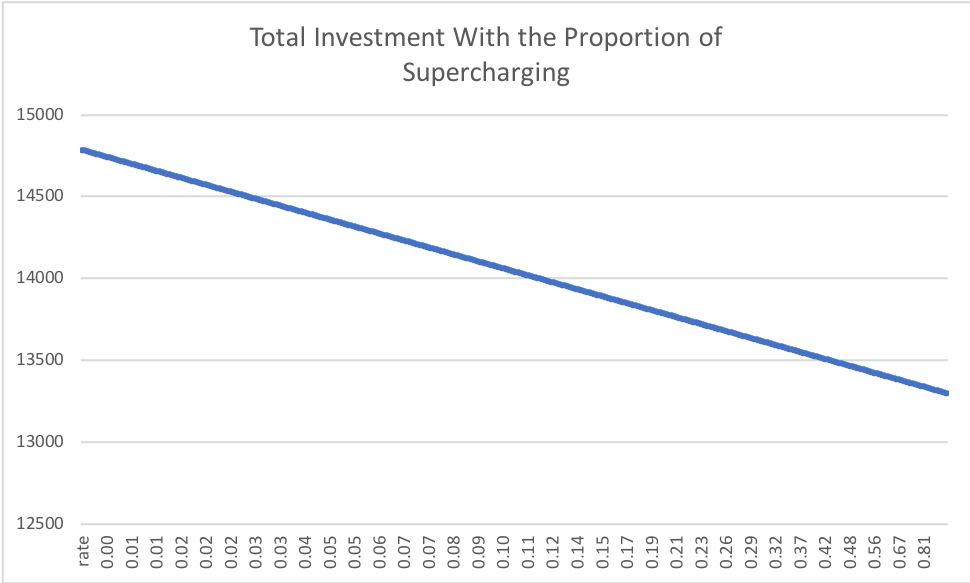
\includegraphics[width=\linewidth]{task1_1.png} \\
\caption{Total Investment With the Proportion of Supercharging} \label{fig:Total Investment With the Proportion of Supercharging}
\end{minipage}
\hspace{1ex}
\begin{minipage}[t]{0.5\textwidth}  
\centering  
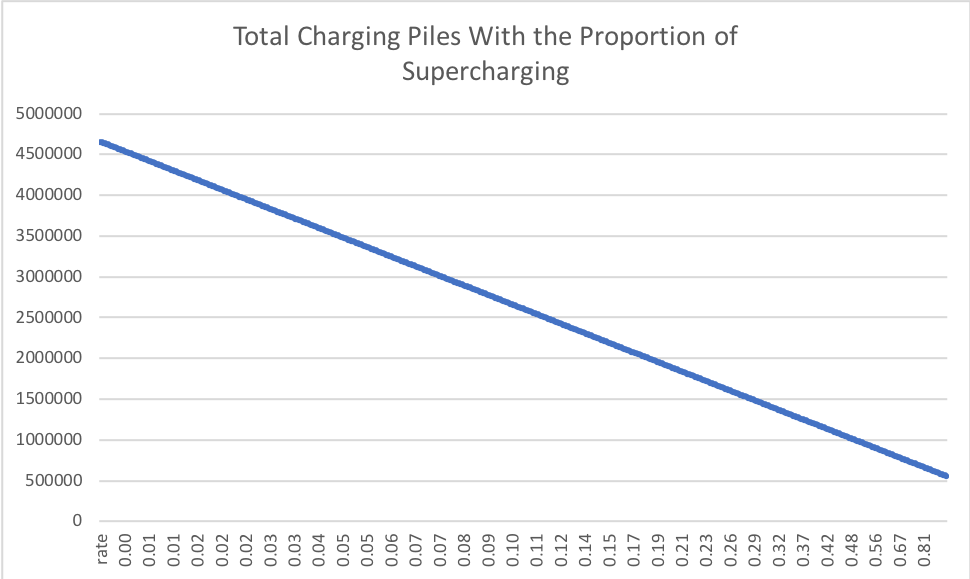
\includegraphics[width=\linewidth]{task1_2.png}\\
\caption{Total Charging Piles With the Proportion of Supercharging}  \label{fig:Total Charging Piles With the Proportion of Supercharging}
\end{minipage}  
\end{figure} 

\par Get a single destination charger cost of 2900\$, a single supercharger cost of 22000\$. We adjust the supercharger in the total number of charging pile ratio, get the result in Figure \ref{fig:Total Investment With the Proportion of Supercharging},\ref{fig:Total Charging Piles With the Proportion of Supercharging}. With the supercharger accounting, the total number of piles and cost of charging piles needed to be established are declining, so consider building all the supercharger.

\par Therefore, 558,719 superchargers should be established in the towns and cities, requiring a total investment of 12,324.7 million dollars.

\subsubsection{Charging Station Design For Highway}

\textbf{Charging Station Number Calculation}

\par According to U.S. law, the distance between two adjacent service areas on the expressway should be more than 40KM and less than 100 km\upcite{fuwuquguiding} . Therefore, we set the charging station to 70 km. Since the total freeway mileage in the United States is 358866 km, a total of 5126 charging stations need to be set up.


\textbf{Charging station scale calculation}

Through the access to information, the total length of the freeway in California is 6519 km and the average daily traffic volume is 1.98 million. According to the survey, the probability of small cars entering the service area is 0.06, and it can be calculated that there are 1275 vehicles per charging station per day on average Into (calculation process as shown in formula \ref{us-size}).

\begin{equation}
	\label{us-size}
	\frac{1980000 \quad cars} {6519 \quad km} \times 70 \quad km \times 0.06 = 1275 \quad cars/day
\end{equation}

Get the parameters in the queuing system: $ \lambda = 1275 \quad cars/day $,$\mu = 33.1 \quad cars/day$ The results calculated by the model are shown in the following table \ref{tab:Charging pile Number With Average Waiting Time}.



\begin{table}[h]
\centering
\caption{Chargers Number With Average Waiting Time}\label{tab:Charging pile Number With Average Waiting Time}
\begin{tabular}{cc|cc}
\toprule
  Server Number & Average Waiting time &  Server Number & Average Waiting time \\
\midrule
40 & 0.3638 H & 41 & 0.1753 H \\
42 & 0.0998 H & 43 & 0.0613 H \\
44 & 0.0391 H & 45 & 0.0255 H \\
46 & 0.0168 H & 47 & 0.0111 H \\
\bottomrule
\end{tabular}
\end{table}


\subsubsection{Charging Station Design Conclusion}


\par Tesla is on track to allow a complete switch to all-electric in the US.
\par The number of Tesla charging stations is growing and there are many more building plans, and the number of supercharging stations has achieved a breakthrough from 0 to 1000 in three years, so it can be proved that Tesla is on track to allow a complete switch to all-electric in the US.

\par If the United States transforms into an all-electric vehicle in an instant, it is necessary to establish 558719 supercharging stations in the city and construct 5126 highway charging stations. The scale of the highway charging station should be selected from Table \ref{tab:Charging pile Number With Average Waiting Time} according to the financial burden and service satisfaction. The cheapest option (40 supercharger per highway charging station) costs\upcite{chongdianzhuangchengben} 29 billion \$.



\section{Task 2: Ireland 's Charging Network and Electric Vehicles}

\par In task 2, we chose Ireland for analysis.

\subsection{A: Hierarchical Charging Station Layout Model Based on Web Search \& Voronoi Diagram}

\subsubsection{Establishment of the Model}

\subsubsection*{Step-by-step Charging Station Distribution Design Model}

\par Because of the shortcomings of computationally complex (ie unfeasible) computations of charging station distribution directly at the national level, we propose a step-by-step charging station distribution design model that divides the charging station distribution into four layers as follows:

\begin{itemize}
	\item Level 1: This level combined with task 1 to calculate the total number of charging stations and the scale should be established. And calculate the number and size of charging stations required for each Irish county.
	\item Level 2: For each city, after the image processing, divide the grid, the grid as a candidate for the establishment of charging station location.BFS algorithm used to ensure that the various charging stations as much as possible coverage of the city at the same time each charging station cross-service range May be selected under the premise of the establishment of the charging station lattice points. Using Voronoi diagram to calculate the specific service for each charging station.
\end{itemize}

\subsubsection*{Hierarchical Charging Station Layout Model Based on Web Search}

\par Breadth-first search (BFS) is one of the easiest graph search algorithms. It is a blind search method that systematically expands and examines all the nodes in the graph to find the result.

\par By query information to get the charging station service range of $0.9 \sim 1.2 km$, in order to ensure maximum coverage and minimum service range overlap, we define the distance between any two charging stations are greater than 2 km, for the selected city, a network of 100 meters intervals Grid division.

\par We search for an optional set of grid points by the BFS algorithm and select an optional grid point (station location) under the constraints of meeting the constraints.

\subsubsection*{Service Area Calculation Model Based on Voronoi Diagram}

The Voronoi Diagram\upcite{voronoi} we use ultimately determines the service area of the charging station found by the grid search.

\textbf{Build Voronoi Diagram}

\par Using the Delaunay triangulation algorithm\upcite{voronoi2} , Mr. into its dual Delaunay triangulation, and then find each triangle triangle circumcircle center, and finally connect the adjacent triangles of the circumcenter of the circle to form a triangular vertex for the polygons network. As shown in figure \ref{fig:task2a_v_step1},\ref{fig:task2a_v_step2},\ref{fig:task2a_v_step3}.


\begin{figure}[htbp]  
\centering
\begin{minipage}[t]{0.2\textwidth}
\centering  
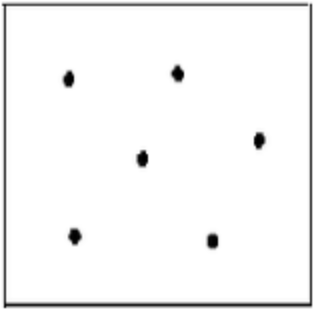
\includegraphics[width=\linewidth]{task2a_v_step1.png} \\
\caption{Step 1} \label{fig:task2a_v_step1}
\end{minipage}
\hspace{1ex}
\begin{minipage}[t]{0.2\textwidth}
\centering  
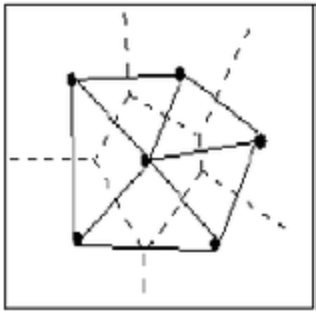
\includegraphics[width=\linewidth]{task2a_v_step2.png} \\
\caption{Step 2} \label{fig:task2a_v_step2}
\end{minipage}
\hspace{1ex}
\begin{minipage}[t]{0.2\textwidth}  
\centering  
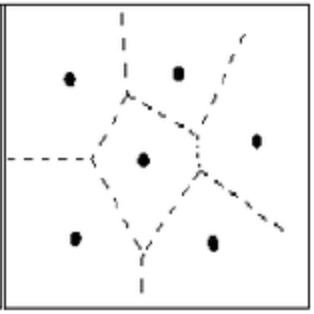
\includegraphics[width=\linewidth]{task2a_v_step3.png}\\
\caption{Step 3}  \label{fig:task2a_v_step3}
\end{minipage}  
\end{figure} 

\par The steps to create a Voronoi diagram are: 

\begin{enumerate}
	\item Discrete points automatically build triangular network, that is, to build Delaunay triangulation. For the discrete points and the triangle formed, record which three discrete points each triangle is made of.
	\item  Calculate the circle center of the circumscribed circle of each triangle and record it.
	\item Traversing the triangular linked list to find the adjacent triangles $Tri_A$, $Tri_B$ and $Tri_C$ coedge with the current triangle p\_Tri trilateral.
	\item If found, connect the outer circle of the found triangle with the outer circle of p\_Tri, and save it in the Vino side chain list. If you can not find, then find the outermost perpendicular perpendicular to the voxel raytraced in the list.
	\item Traversal over, all the Voronoi edges are found, and the Voronoi diagram is drawn according to the edge.
\end{enumerate}



\textbf{Delaunay Triangulation Generation}

\par The key to establishing Voronoi diagram is the generation of Delaunay triangulation.


\par The steps to generate Delaunay triangulation are: 

\begin{enumerate}
	\item Construct a super triangle, containing all the scatter points, into the triangle linked list.
	\item Insert the scattered points of the set of points in turn, find the triangle whose insertion circle contains the insertion point (called the influence triangle of this point) in the triangle linked list, delete the common edges that affect the triangle, insert the insertion point All the vertices are joined together to complete the insertion of a point in the Delaunay Triangle linked list. (show in figure \ref{fig:Detailed Explanation of Step Two} From left to right: Insert P; Decide how to link P; Delete edge AB;Make new triangle).
	\item According to the optimization criterion, the local newly formed triangle is optimized. Place the resulting triangle in the Delaunay Triangle linked list.
	\item Loop through step 2 above until all the scatter points have been inserted.
\end{enumerate}


\begin{figure}[htbp]  
\centering
\begin{minipage}[t]{0.2\textwidth}
\centering  
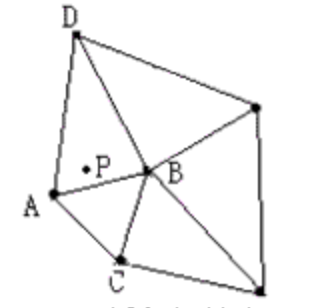
\includegraphics[width=\linewidth]{insertP.png} \\
%\caption{Insert node P} 
\label{fig:Insert node P}
\end{minipage}
\hspace{1ex}
\begin{minipage}[t]{0.2\textwidth}
\centering  
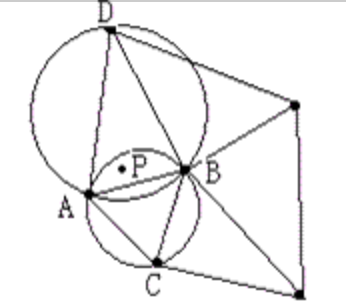
\includegraphics[width=\linewidth]{linkP.png} \\
%\caption{Decide how to link P} 
\label{fig:Decide how to link P}
\end{minipage}
\hspace{1ex}
\begin{minipage}[t]{0.2\textwidth}
\centering  
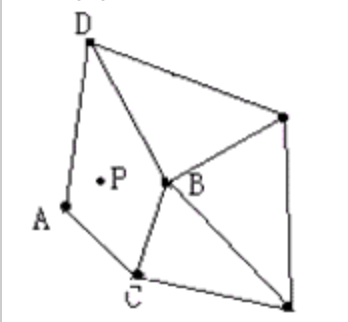
\includegraphics[width=\linewidth]{deleteAB.png} \\
%\caption{Delete edge AB} 
\label{fig:Delete edge AB}
\end{minipage}
\hspace{1ex}
\begin{minipage}[t]{0.2\textwidth}  
\centering  
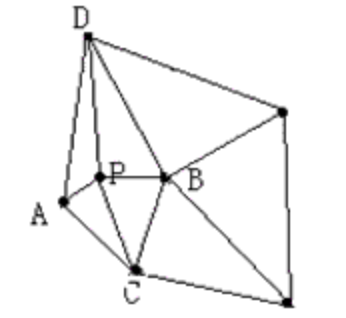
\includegraphics[width=\linewidth]{newTri.png}\\
%\caption{Make new triangle}  
\label{fig:Make new triangle}
\end{minipage}  

\caption{Detailed Explanation of Step Two}
\label{fig:Detailed Explanation of Step Two}
\end{figure} 


\subsubsection{Calculation and Analysis}

\subsubsection*{Level 1: Country and County}

\textbf{Charging Station Number For Urban, Suburban, Rural Area}

\par Based on the task 1 method, we got 263,1092 car ownership in Ireland\upcite{aierlantongji} , and the national average car mileage (car/year) was 18,411 km. According to the formula \ref{2al1-1}, the average daily car needs to be charged accounted for 9.27\% of the total car. , Calculated according to formula \ref{2al1-2} should be built in the town of 7370 supercharger. 

\begin{equation}
	\label{2al1-1}
	\frac{18411 \quad km/car \cdot year}{544 \quad km \times 365} = 0.09271 
\end{equation}

\begin{equation}
	\label{2al1-2}
	\lceil \frac{0.09271 \times 2631092}{33.1 \quad car/charger} \rceil= 7370
\end{equation}

\par As table \ref{tab:2015 Ireland Cars Number Statistics} shows the proportion of car ownership in Irish urban, suburbs and rural areas, the proportion of charging stations in the final three regions is 0.61, 0.09, 0.29

\begin{table}[h]
\centering
\caption{2015 Ireland Cars Number Statistics}\label{tab:2015 Ireland Cars Number Statistics}
\begin{tabular}{c|ccc}
\toprule
 & Urban & Suburban & Rural Area\\
\midrule
Proportion & 0.6159 & 0.0914 & 0.2926 \\
\bottomrule
\end{tabular}
\end{table}
      

\textbf{Charging Station Number For Highway}

\par According to the inquired data, the total mileage of the Irish National Freeway is 5305 km and the traffic volume is 1.2524 million vehicles/day. According to the method of task 1, the arrival flow of the charging station is calculated as $ \lambda = 991.53 \quad cars/day $. And the number of charging stations is 76.

\par Then use queuing theory model to get the number of charging station's superchargers alternative list as follow table \ref{tab:Charging pile Number With Average Waiting Time Ireland}


\begin{table}[h]
\centering
\caption{Chargers Number With Average Waiting Time}\label{tab:Charging pile Number With Average Waiting Time Ireland}
\begin{tabular}{cc|cc}
\toprule
  Server Number & Average Waiting time &  Server Number & Average Waiting time \\
\midrule
31 & 0.5583 H & 32 & 0.2243 H \\
33 & 0.1164 H & 34 & 0.0671 H \\
35 & 0.0406 H & 36 & 0.0252 H \\
37 & 0.0158 H & 38 & 0.0101 H \\
\bottomrule
\end{tabular}
\end{table}

\textbf{Country's Charging Station Design Conclusion}


\par If Ireland transforms into an all-electric vehicle in an instant, it is necessary to establish 7370 supercharging stations in the city and construct 76 highway charging stations. The scale of the highway charging station should be selected from Table \ref{tab:Charging pile Number With Average Waiting Time Ireland} according to the financial burden and service satisfaction. The cheapest option (31 supercharger per highway charging station) costs 213.97 million cities, The proportion of urban, suburbs and rural areas is 0.61, 0.09, 0.29\$.


\par Regardless of the impact of the highway, the method of calculating the number of charging poles in the city is the same as task 1.
\par Based on the queried data of the car ownership in each county, the number of supercharger that each county needs to establish is as shown in the following table \ref{tab:Sub-regional charging pile demand Ireland} and figure \ref{fig:Sub-regional charging pile demand}.

\begin{table}[h]
\centering
\caption{Sub-Regional Chargers Demand}\label{tab:Sub-regional charging pile demand Ireland}
\begin{tabular}{cc|cc|cc|cc}
\toprule
  County & Number &  County & Number & County & Number &  County & Number \\
\midrule
Carlow	&105	&Longford	&65 &Cavan	&121	&Louth	&172\\
Clare	&205	&Mayo	&228 & Cork	&900	&Meath	&294\\
Donegal	&244	&Monaghan	&101 & Dublin	&1795	&Offaly	&126\\
Galway	&409	&Roscommon	&119 & Kerry	&259	&Sligo	&107\\
Kildare	&342	&Tipperary	&284 & Kilkenny	&163	&Waterford	&194\\
Laois	&124	&Westmeath	&148 & Leitrim	& 56	& Wexford 	&267\\
Limerick	&310	&Wicklow	&229\\
\bottomrule
\end{tabular}
\end{table}

\begin{figure}[!h]
\small
\centering
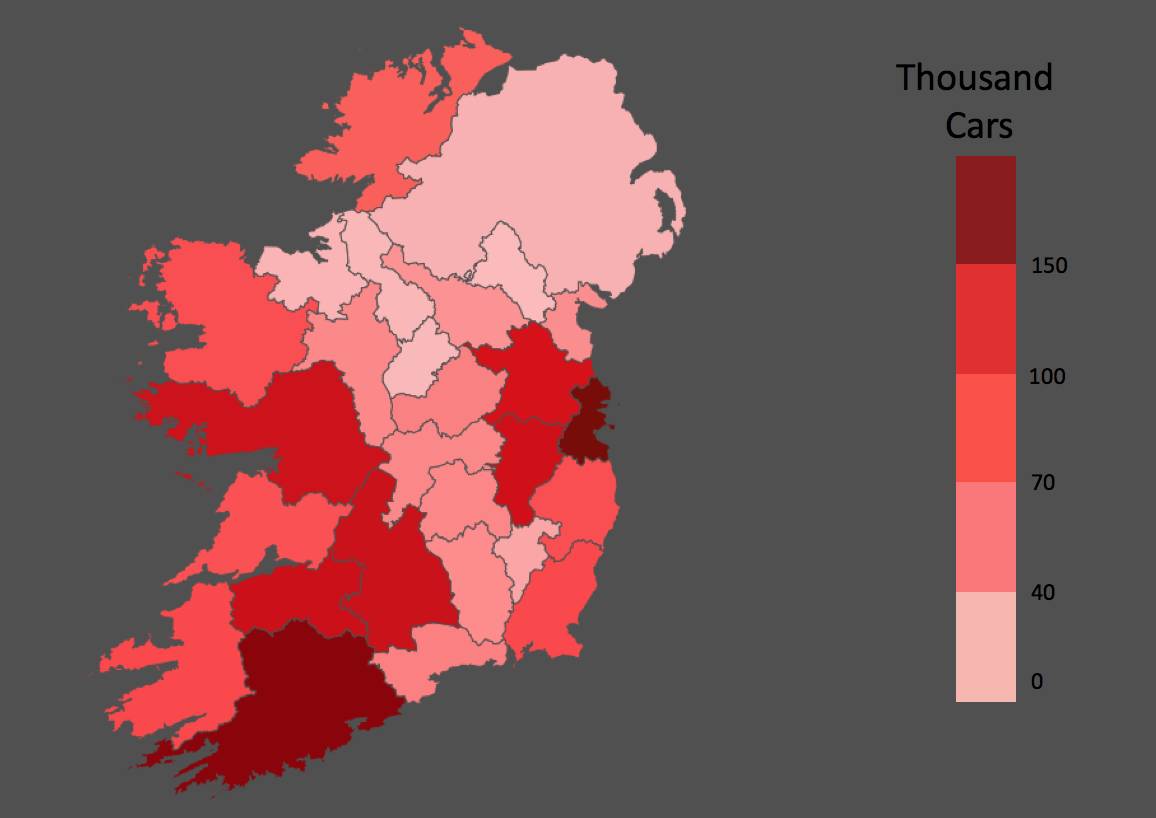
\includegraphics[width=9cm]{map.png}
\caption{Sub-regional charging pile demand} \label{fig:Sub-regional charging pile demand}
\end{figure}

\newpage
\subsubsection*{Level 2: City}

\par Urban Meshing Based on Image Processing - Confirming the Location Range of Charging Stations. Take County Dublin as an Example: Divide the city into grids of $ 218 \times 256 $ using scale and city real estate. There's four step to build the grids as flowing:

\begin{enumerate}
	\item Get an administrative map of Dublin City from Google Maps(figure \ref{fig:administrative map of Dublin}).
	\item Boundary detection and extraction of the map.Then according to the scale division of the grid width of 100 meters(figure \ref{fig:Boundary Map of Dublin}).
	\item Fill to get the white area as a grid of grid points to build a charging station(figure \ref{fig:Filled Map of Dublin}).
	\item Grid search, in accordance with the restrictions to be resolved 64 grid points(Part of the selected grid points such as: (49,87),(54,228),(54,256),(56,26)) as the charging station construction location center(figure \ref{fig:Selected Point Map of Dublin}).
\end{enumerate}


\begin{figure}[htbp]  
\begin{minipage}[t]{0.5\textwidth}
\centering  
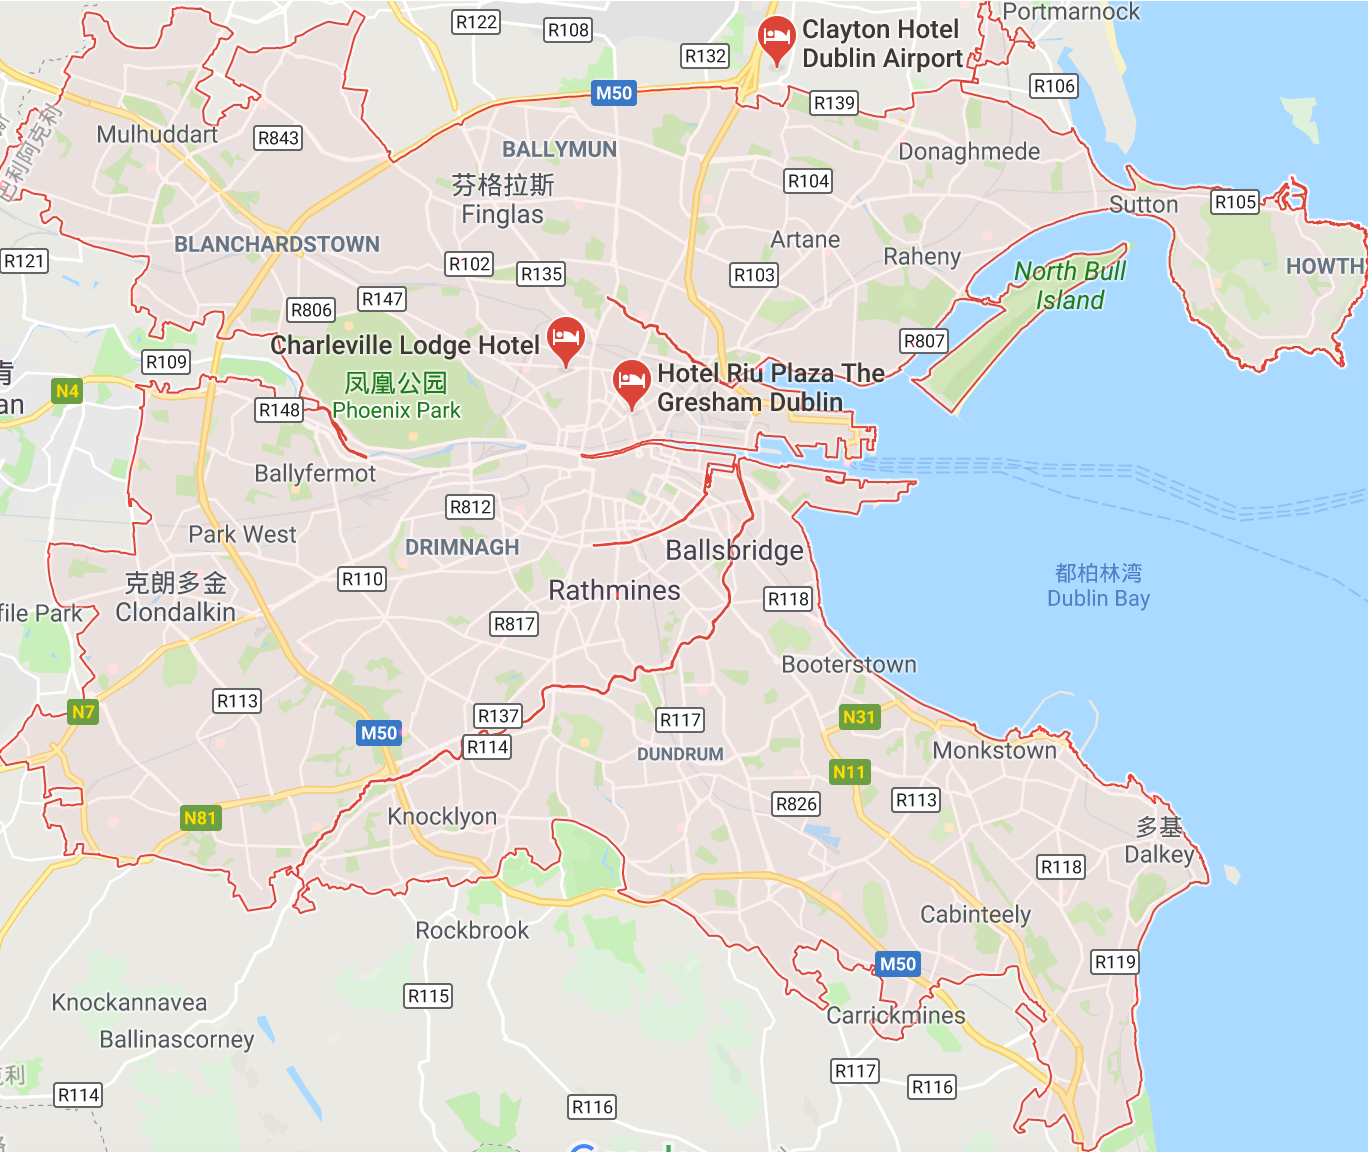
\includegraphics[width=\linewidth]{task2a_0.png} \\
\caption{Administrative Map of Dublin} \label{fig:administrative map of Dublin}
\end{minipage}
\hspace{1ex}
\begin{minipage}[t]{0.5\textwidth}  
\centering  
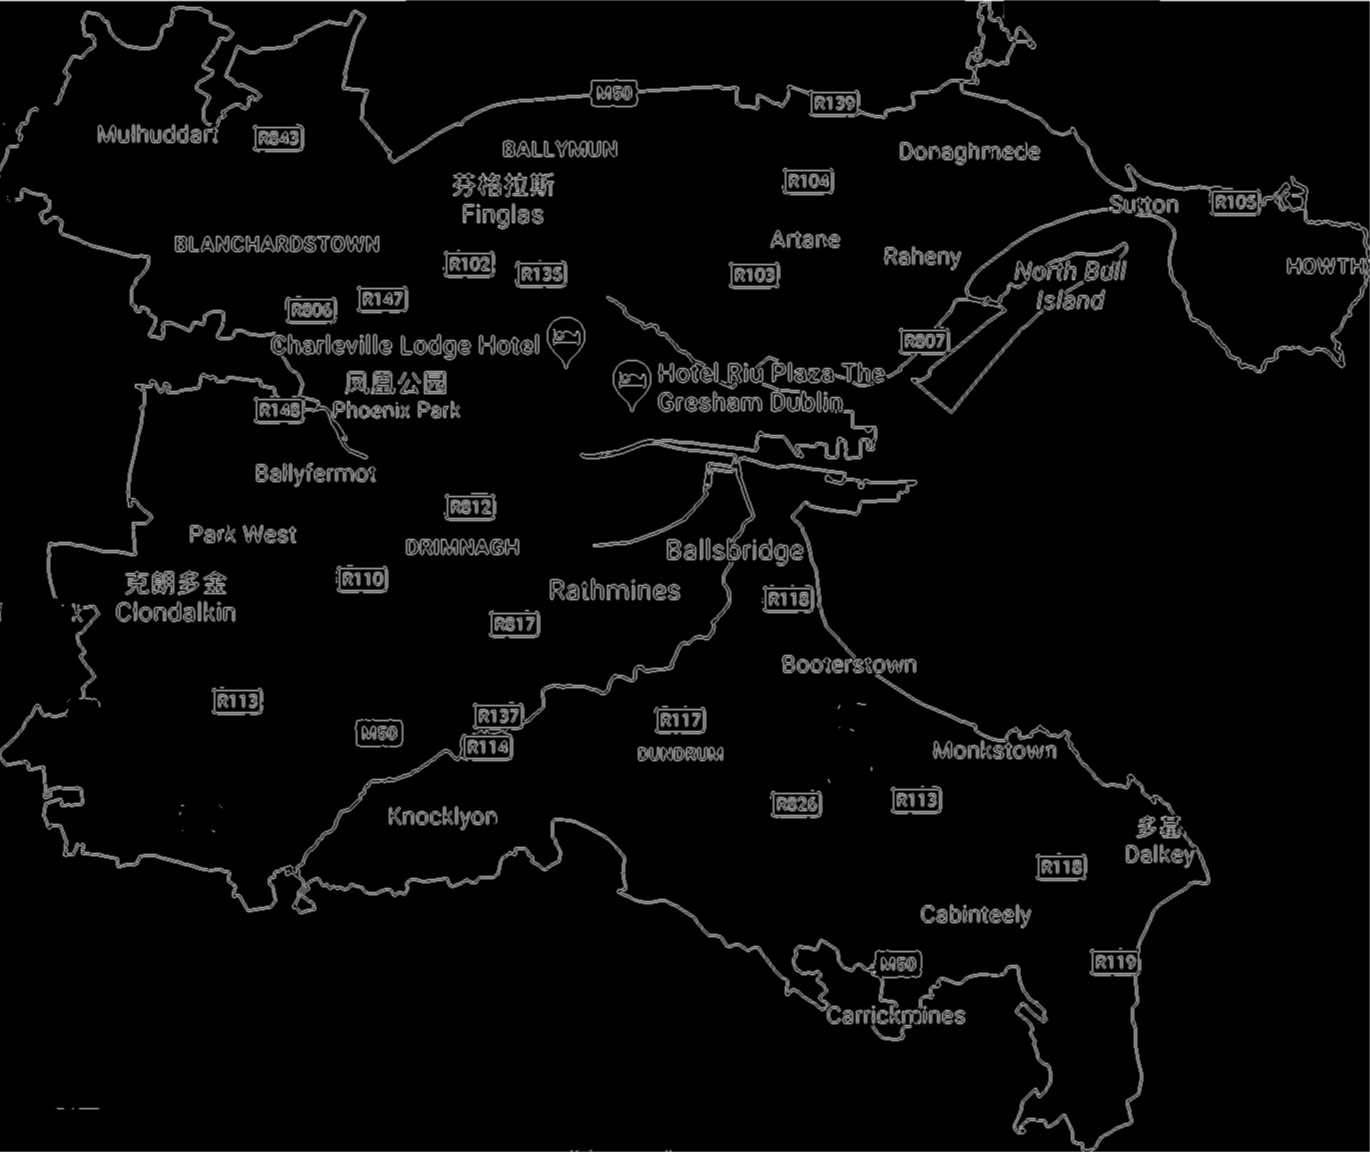
\includegraphics[width=\linewidth]{task2a_2.png}\\
\caption{Boundary Map of Dublin}  \label{fig:Boundary Map of Dublin}
\end{minipage}  
\end{figure} 

\begin{figure}[htbp]  
\begin{minipage}[t]{0.5\textwidth}
\centering  
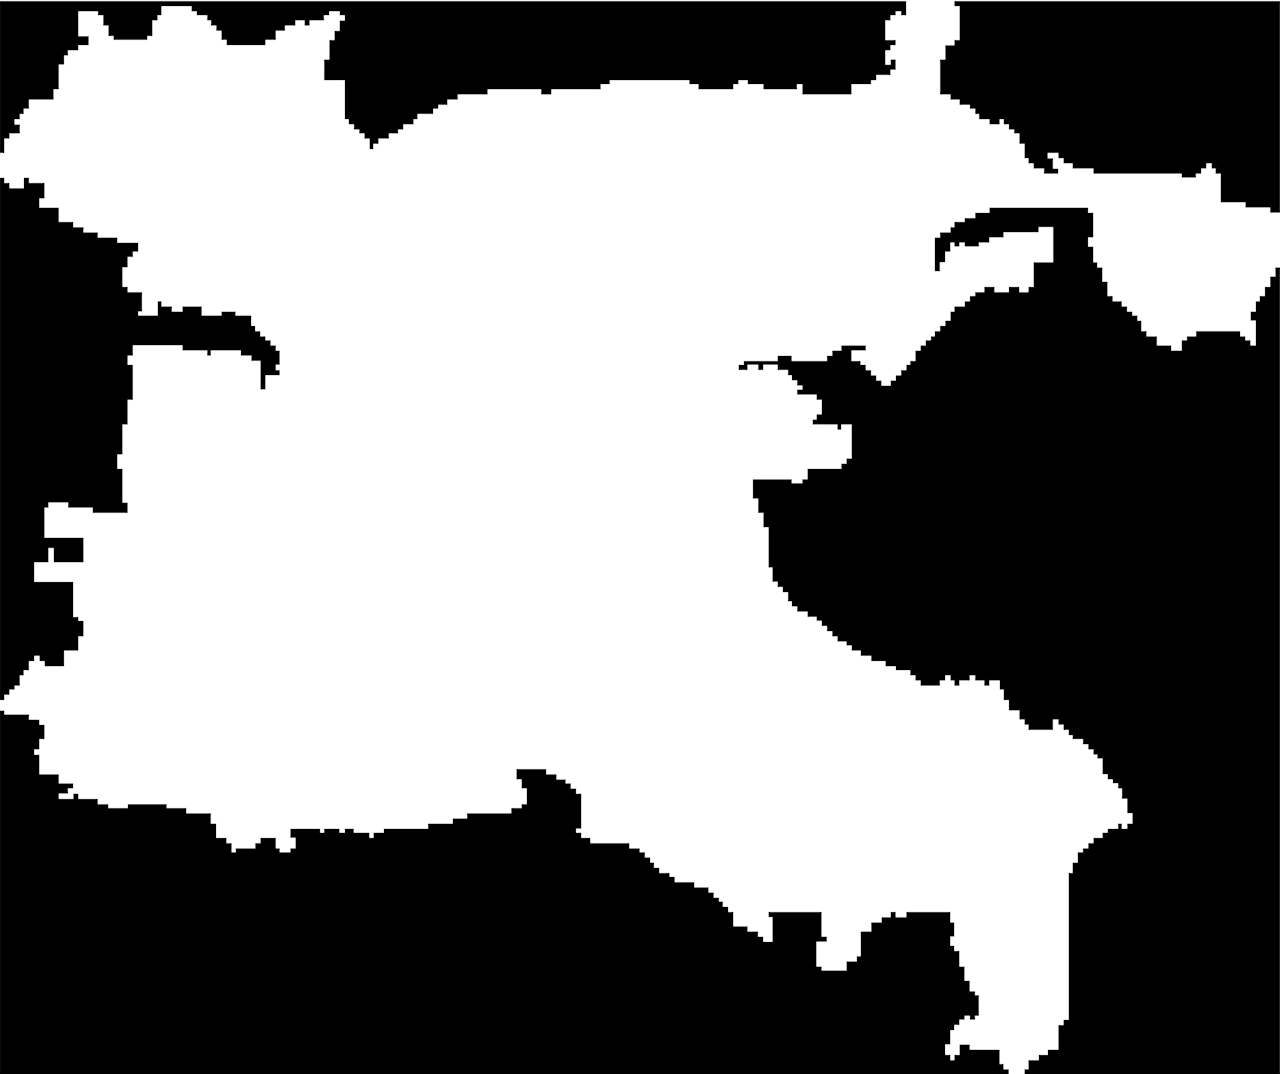
\includegraphics[width=\linewidth]{task2a_1.png} \\
\caption{Filled Map of Dublin} \label{fig:Filled Map of Dublin}
\end{minipage}
\hspace{1ex}
\begin{minipage}[t]{0.5\textwidth}  
\centering  
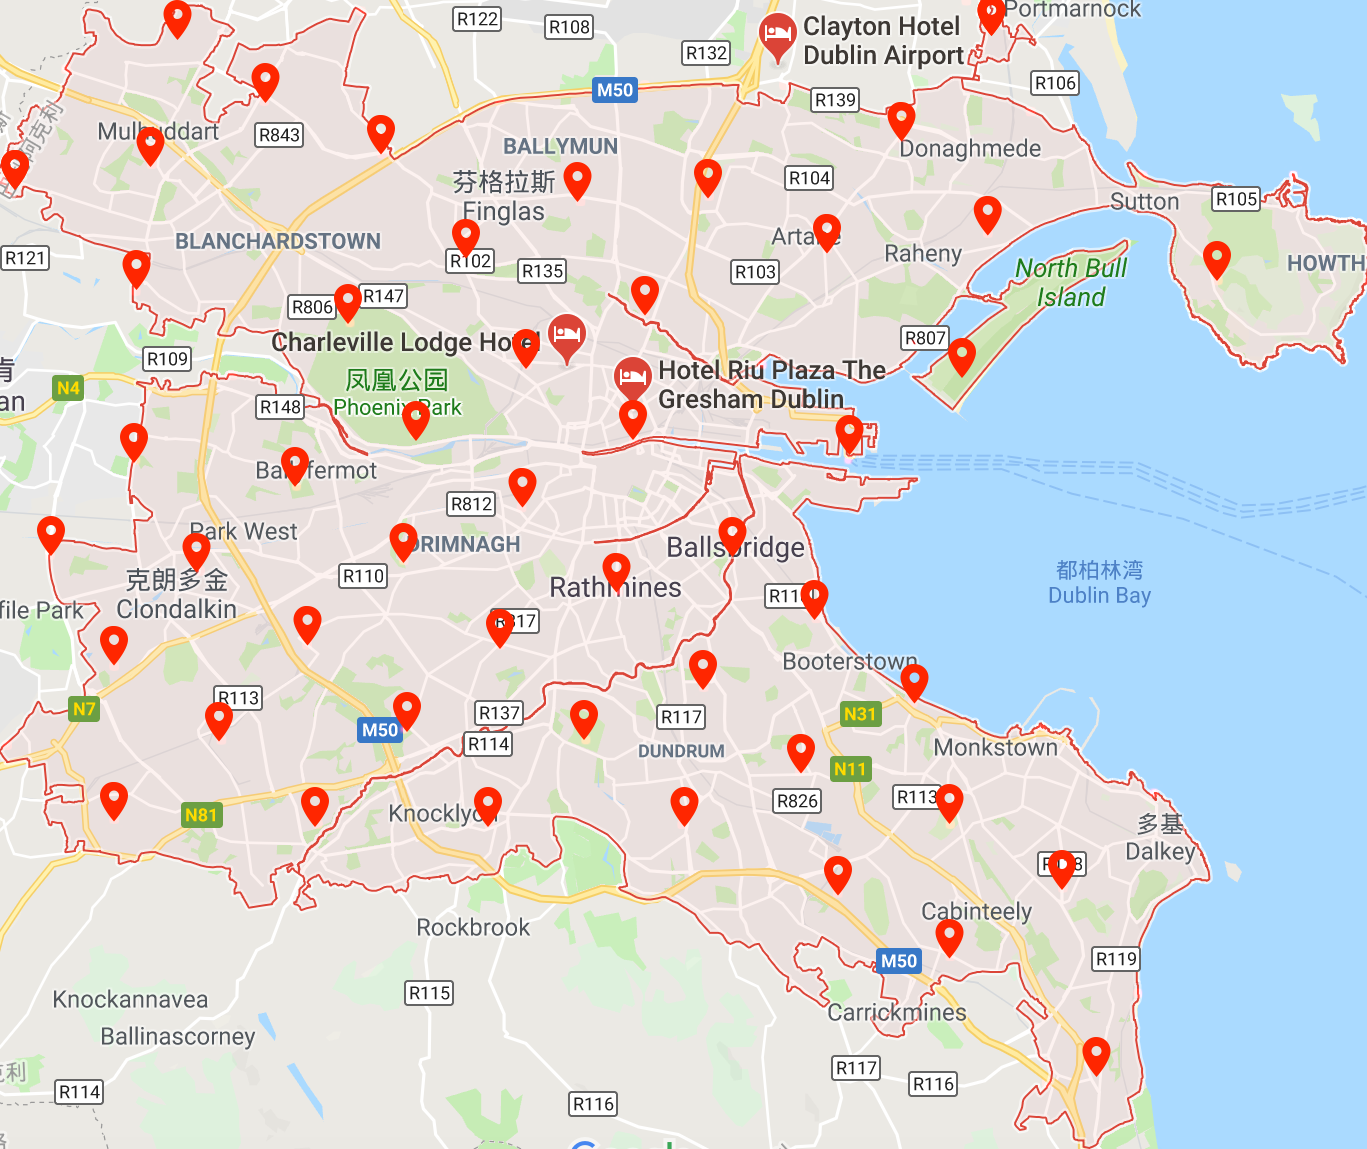
\includegraphics[width=\linewidth]{task2a_3.png}\\
\caption{Selected Point Map of Dublin}  \label{fig:Selected Point Map of Dublin}
\end{minipage}  
\end{figure} 


\par According to the Voronoi diagram to determine the specific service range of each charging station. As shown in Figure \ref{fig:Delaunay triangle of Dublin} is the Delaunay triangle of level 3 selected points.Figure \ref{fig:Voronoi diagram of Dublin} shows the final Dublin city distribution of charging stations and their corresponding service range.

\begin{figure}[htbp]  
\begin{minipage}[t]{0.5\textwidth}
\centering  
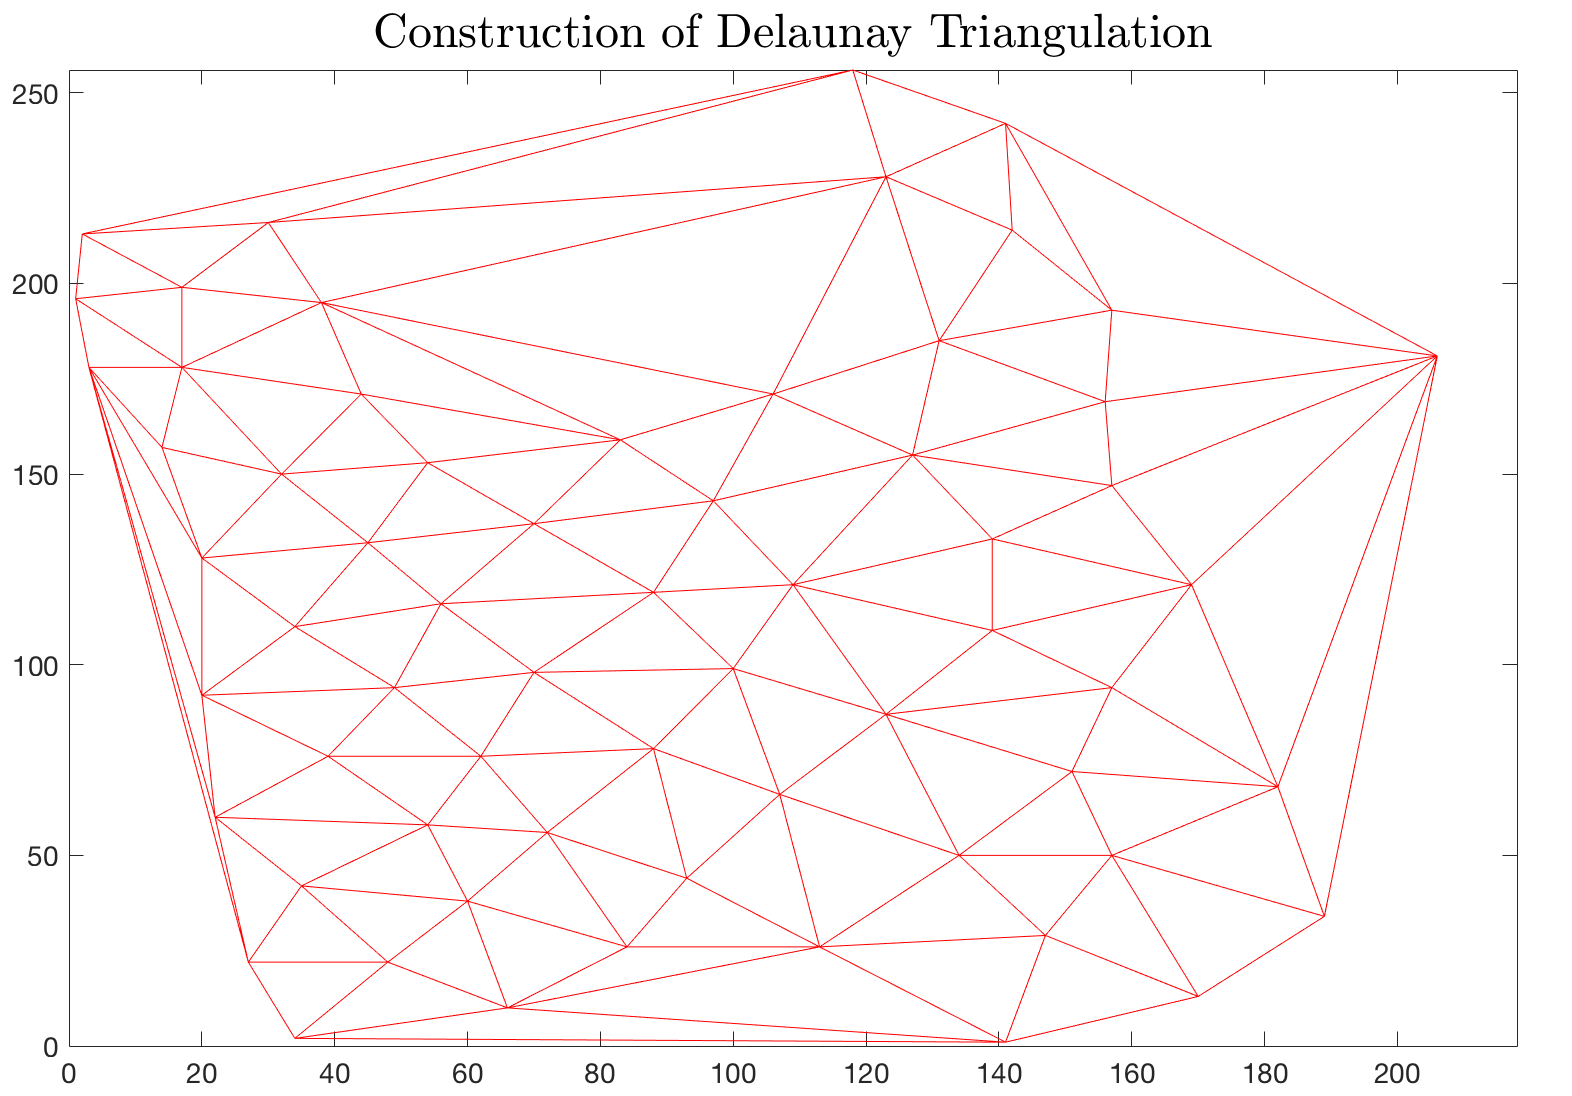
\includegraphics[width=\linewidth]{task2a_delaunay.png} \\
\caption{Delaunay triangle of Dublin} \label{fig:Delaunay triangle of Dublin}
\end{minipage}
\hspace{1ex}
\begin{minipage}[t]{0.5\textwidth}  
\centering  
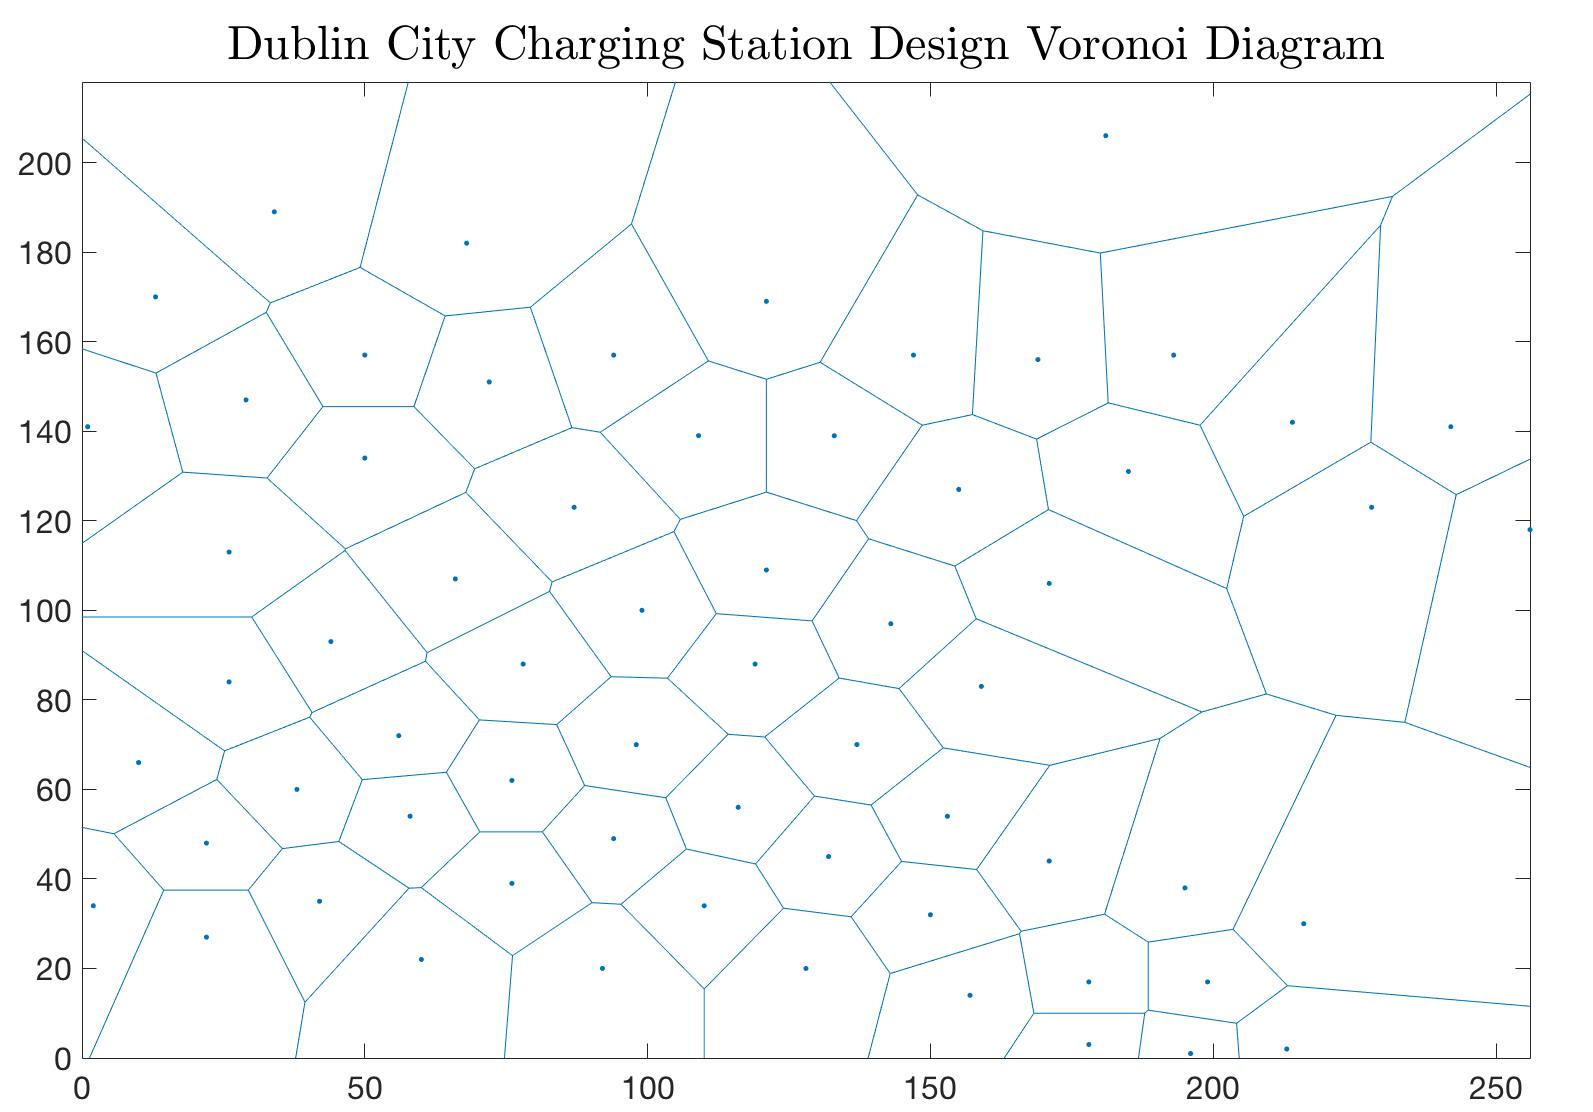
\includegraphics[width=\linewidth]{task2a_voronoi.png}\\
\caption{Voronoi diagram of Dublin}  \label{fig:Voronoi diagram of Dublin}
\end{minipage}  
\end{figure} 

\subsection{B: Charging Network Development Proposals.}

\subsubsection{Establishment of the Model}

\subsubsection*{Charging stations in different regions to develop priorities}

\par We use the Gini coefficient\upcite{gini} to measure the disparity in the distribution of income within each country.If the Gini coefficient of the country is greater than the median of the Gini coefficient of each country in the world, we think the country's domestic income distribution is significantly different and should select the one with superior urban and rural development Give priority to development.If the Gini coefficient of the country is less than the median of all countries in the world, the difference between urban and rural areas in the country is not significant, and mixed development should be chosen.

\subsubsection*{Electric cars and charging stations development priorities}


\par In order to measure whether the country can bear the development mode of buying cars after building chargers first. We analyzed the amount of national power generation and investment in national infrastructure construction, which is not possible due to the rapid development in some countries but the current economic output or insufficient power generation In the same year, investment was completed, but basic conditions for the popularization of electric vehicles could be achieved in a few years. Therefore, we introduced a gray prediction system to predict the power generation and other related data in the coming years through the GM (1,1) algorithm.

\textbf{GM (1,1)  Data Prediction Model}

\par The traditional GM (1,1) model\upcite{gm} is composed of a differential equation containing univariate.

\par Let $X^{(0)}=[x^{(0)}(1), x^{(0)}(2),\cdots ,x^{(0)}(n)]$ , $X^{(1)}=[x^{(1)}(1), x^{(1)}(2),\cdots ,x^{(1)}(n)]$ , $Z^{(1)}=[z^{(1)}(1), z^{(1)}(2),\cdots ,z^{(1)}(n)]$ , where $x^{(1)}(k) =  \sum\limits_{i=1}^k x^{(1)}(i)$ and $z^{(1)}(k) = \frac{x^{(0)}(k) + x^{(0)}(k+1)}{2}$ , then $x^{(0)}(k) + a z^{(1)}(k) = b$ is called the GM(1,1) model. The parameter $a$ is called the development coefficient, and the parameters $b$ is called the grey action quantity.
 
Then, we can get the time responded function of GM(1,1) model.

\begin{equation}
\hat{x}^{(1)}(k+1) = (x^{(0)}(1) - \frac{b}{a})e^{-a k} + \frac{b}{a} \qquad k = 1, 2, \cdots, n
\end{equation}
and the restored function of $x^{(0)}(k + 1)$ can be given by

\begin{equation}
\hat{x}^{(0)}(k+1) = (1 - e^a)(x^{(0)}(1) - \frac{b}{a})e^{-a k} \qquad k = 1, 2, \cdots, n
\end{equation}

\par In which, $\hat{x}^{(1)}(k)$ is the simulative value of  $x^{(1)}(k)$, and  $\hat{x}^{(0)}(k)$ is simulative value of $x^{(0)}(k)$

\par Without external interference, we know that the population and GDP was exponential growth. But this model will produce a continuously simulative deviation when simulating a homogeneous-exponent sequence. Because the unequal conversion between the discrete difference equation and continuous differential equation. So we learn from C.I.Chen\upcite{}. The Discrete GM(1,1) Model as follows:
\begin{equation}
\hat{x}^{(1)}(k+1) = (x^{(0)}(1) - \frac{b}{a})(\frac{2 - a}{2 + a})^k+ \frac{b}{a} \qquad k = 1, 2, \cdots, n
\end{equation}
\begin{equation}
\hat{x}^{(0)}(k+1) = (1 - \frac{2 + a}{2 - a})(x^{(0)}(1) - \frac{b}{a})(\frac{2 - a}{2 + a})^k \qquad k = 1, 2, \cdots, n
\end{equation}
\par Use least squares to solve $a$ and $b$. Put it into the prediction formula. We can get the predictive value $X^{(1)}$, and the analog value of $X^{(0)}$.\\



\subsubsection{Calculation and Analysis}


\par The median Gini coefficient for all countries in the world was 37.4. The Gini coefficient for Ireland was 32.5, indicating that the economic gap between urban and rural areas in Ireland is relatively small and should choose the mixed  develop plan. 

\par Based on the calculation of task 2A and the related data found, we determine the total power consumption of the current year excluding the electric load brought by the electric vehicle: 29,870,140 MWH. If all cars were converted to electric vehicles, an extra 7,747,003 MWH of electrical energy would have to be absorbed.

\par The total generation of power in the current year is 32,953,657 MWH, which can not meet the electricity demand of the first charging pile. By the GM (1,1) algorithm, it is estimated that after three years the national power generation is estimated to be 37,949,293MWH, which can meet the entire power demand. Considering the time it takes to build a chargers, we think Ireland can afford the electrical load that the first built chargers would bring.

\par The current year Irish infrastructure investment is estimated to be 21 billion dollars, much larger than the cost of build chargers(213.97 million dollars).

\par In summary, we think Ireland should choose to build chargers before buy cars' development plan.

\subsubsection{Conclusion}

Ireland may choose the plan that develop cities and rural areas both and build the chargers before buy the cars.


\subsection{C: Price Distribution Movement Model Based on Gray Prediction}

\subsubsection{Factors limiting the development of electric vehicle}


\textbf{Purchasing Power}

\par In the industrial system of manufacturer's production, national power supply and people's purchase and use, we draw the conclusion from the CNDP model that the national grid and economic power in Ireland will not become the restriction that restricts the establishment of power stations and the promotion of electric vehicles. Thanks to the interest-driven and policy, the productivity of manufacturers will not become a bottleneck restricting the development of electric vehicles, neither. Therefore, people's purchasing power becomes an important factor restricting the development of electric vehicles. People's purchasing power is mainly related to the growth of GDP per capita and the relation between per-capita GDP and the selling price of electric vehicles.            

\begin{itemize}
	\item \textbf{Per capita GDP growth}
		\par Per capita GDP growth will increase people's purchasing power. In this model we use the GM (1,1) algorithm to predict GDP per capita over the coming period.
	\item \textbf{The relation between per-capita GDP and the selling price of electric vehicles}
		\par Per capita GDP inevitably affects the distribution of selling prices and sales volume of electric vehicles. Through the analysis of the existing data, we find that when the distribution curve of the cars almost unchanged, but with the GDP moving, it also move g. 
		\par In the same situation of the distribution of electric vehicles, the increase of purchasing power will lead to more sales of electric vehicles and the expansion of the proportion of electric vehicles in the market.
\end{itemize}


\textbf{The Will to Buy Electric Cars}

\par For the benefits electric cars have such as environmental protection and energy saving, compared with the same price of gasoline vehicles in the market electric cars have more advantages. Meanwhile, the government has introduced a series of incentive policies for electric vehicles to improve the environment, actively promoting electric vehicles and intending to impose a ban on gasoline vehicles. Under the pressure of policies, the vast majority of people will choose electric vehicles when their purchasing power is sufficient.



\subsubsection{Establishment of the Model}


\par Through the analysis of the main influencing factors, we make the following assumptions.

\subsubsection*{Assumptions}
\begin{itemize}
	\item The shape of sales-price  curve is the changeless ,but the values moves equidistantly with the change of per capita GDP.
	\item The price of Electric cars represented by Tesla will not change drastically in following ten years.
	\item When people have enough purchasing power, people will choose to buy electric cars.
\end{itemize}

\subsubsection*{Model Diagram} 

\begin{figure}[!h]
\small
\centering
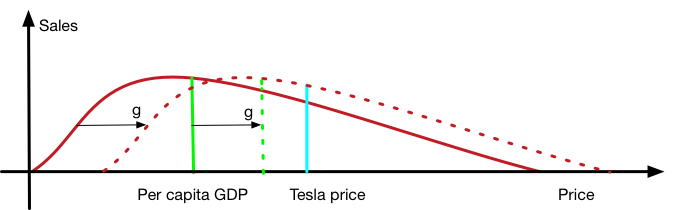
\includegraphics[width=12cm]{task2c_model.png}
\caption{Model Diagram} \label{fig:Model Diagram}
\end{figure}

\par The curve(show in figure \ref{fig:Make new triangle}) of Sales Price shows the distribution of sales in different price, whose shape will not change when Per capita GDP increases by g. But it's value also increases by g.



\subsubsection{Calculation and Analysis}

\par In order to solve this model, we have compiled the computer according to the model Simulation program:
\begin{enumerate}
	\item GM (1,1) algorithm\upcite{gm} is used to forecast GDP per capita in the next 20 years 
		
		\begin{figure}[!h]
			\small
			\centering
			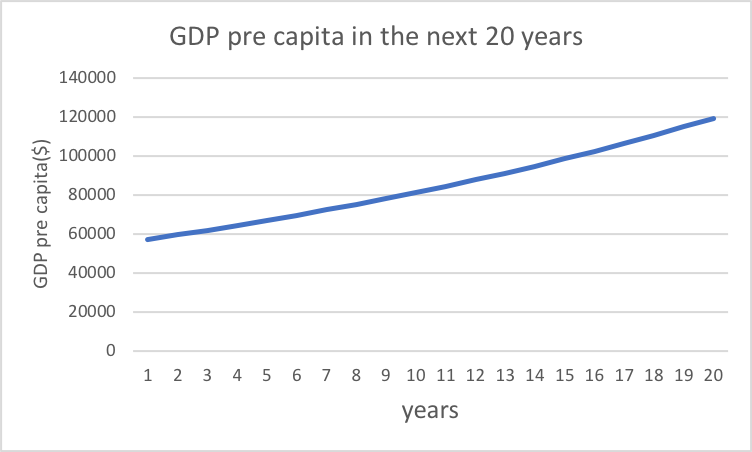
\includegraphics[width=12cm]{task2c-GDPinthenext20years}
			\caption{GDP per capita in the next 20 years} \label{fig:GDP per capita in the next 20 years}
		\end{figure}

	\item According to the change of GDP to solve the annual car sales - price distribution
	\item According to the lowest price of Tesla electric cars, calculate the ratio of electric cars to new cars 
\end{enumerate}

\begin{table}[h]
\centering
\caption{timetable of Electric vehicles proportion}\label{tab:timetable of Electric vehicles proportion}
\begin{tabular}{ccccccccccc}
\toprule
 Year & 1 &2 &3 &4 &5 &6 &7 &8 &9 &10 \\
\midrule
Ratio & 0.23 & 0.27 &	0.38 &	0.45 & 0.54 & 0.67 & 	0.78 & 	0.85 & 	0.93 &	1 \\	
\bottomrule
\end{tabular}
\end{table}


\par From table \ref{tab:timetable of Electric vehicles proportion}, we can see that with the current development trend in Ireland and based on the development model we proposed, it will take about 10 years for electric vehicles to completely replace other energy vehicles.


\section{Task 3: Charging Network Growing \& Evolving Plan Classification System}
\subsection{Establishment of the Model}

\par We summarize two factors that affect the development of different countries. Firstly we consider the distribution of wealth, and use the Gini coefficient to measure the economic gap between urban and rural areas, determine the order of establishing charging stations between urban and rural areas. secondly, we consider the resource, use the power resources and state financial capacity to measure the ability of building charging stations. Decide whether suggest the country to build the chargers first to encourage people buying the cars, or build chargers in response to car purchases.

\par We analyze the Gini Coefficient in 157 countries. Choose the median Gini Coefficient($G_{mid}$) of 157 data as the Classification criteria.
If 
$$G(m)>G_{mid} $$

\par It shows that There is a big economic gap between urban and rural areas in the country. Then we compare the per capita GDP in city and rural areas, if the former is larger than the latter, we suggest the country to build all city-based charging station first, if not, we suggest the country to build all rural charging station first.
If

$$G(m)<G_{mid}$$

\par It shows that there is almost no economic gap between urban and rural areas in the country. We suggest the country can build a mix of both.

\par we use GM(1,1) to predict the electricity resources and the National GDP, the national GDP represent the economic strength of the country. we find that 2.3\% of the National GDP is the investable amount of building charging stations. 

\par Compare the cost of building charging stations with the investable amount, meanwhile, compare the demand for electricity for electric cars with the electricity resources. If the former is greater than the latter in both comparisons, we suggest the country could build the chargers first to encourage people buying the cars, and improve the environment. If not, we suggest the country could build chargers in response to car purchases, which can reduce the country’s burden.




\subsection{Calculation and Analysis}
\par According to our models constructed, we divide the country's program of setting up charging stations into six, the six program is shown in table \ref{tab:6 Types of Plan}.

\begin{table}[h]
\centering
\caption{Six Types of Plan}\label{tab:6 Types of Plan}
\begin{tabular}{ccl}
\toprule
Urban-rural gap & Power Generation \& Investment & Plan\\ 
\midrule
Urban $\gg$ Rural & $\surd$ & City | Chargers\\
Urban $\gg$ Rural &  		 & City | Cars\\
Urban $\ll$ Rural & $\surd$ & Rural | Chargers\\
Urban $\ll$ Rural &  	     & Rural | Cars\\
Urban $\approx$ Rural & $\surd$ & Mixed | Chargers\\
Urban $\approx$ Rural &  & Mixed | Cars\\

\bottomrule
\end{tabular}
\end{table}


\par We select Indonesia to verification our models constructed. We find that the plan of building charging stations is different from Ireland. 
\par Firstly, the Indonesia need build chargers in response to car purchases so that it won’t increase the burden of economic.
\par Secondly, Because the Gini Coefficient is larger than the $G_{mid}$, and the per capita GDP in city is larger than in rural areas, the Indonesia should build the charging stations in cities first.
\par Finally, we find that the personal passenger vehicles need a long time to switch all-electric in Indonesia.

\subsection{Conclusion}

\par We conclude that the key factors of choosing different program of setting up charging stations are: the electricity resources, the National GDP, the economic gap between urban and rural areas.

\section{Task 4: Technology Impact Increasing of Electric Vehicles}
\subsection*{Car-Share and Ride-Share Services}
Car-Share and Ride-Share are convenient ways to travel, which will reduce people's desire to buy new family cars. Obviously, the proportion of electric car in new cars is more than that in the old cars. Thereby, in the first ten years from when electric cars first show up in the market, Car-Share and Ride-Share services will surely slow down the process of electric car replacing gasoline car. However, it will changes, when the first batch electric cars have to be scrapped. In order to visualize this effect, we set data as followed to simulate the proportion of electric vehicles in total vehicles in 30 years.

\begin{itemize}
	\item \textbf{No Car-Share and Ride-Share Service}
		\par Car ownership in last years: 10000;The number of cars scrapped each year: 1000;The number of new cars each year: 1200; The proportion of Electric cars in new cars grow every year by 5\% from 0\%. 
	\item \textbf{With Car-Share and Ride-Share Service}
		\par The number of new cars of each year decrease to 1100 per year with the effect of Car-Share and Ride-Share.
	
\end{itemize}

\begin{figure}[!h]
\small
\centering
\includegraphics[width=9cm]{task4a.png}
\caption{Effect of Car-Share and Ride-Share Service} \label{fig:Effect of Car-Share and Ride-Share Service}
\end{figure}

\par The result show in the figure \ref{fig:Effect of Car-Share and Ride-Share Service}.
\par We could tell car-share and ride-share have little effect in the increasing use of electric vehicles.


\subsection*{Rapid Battery-Swap Stations}

\par Rapid battery-swap stations' service time is obviously much shorter than charging stations. Correspondingly, the rapid battery-swap stations' scale could be smaller which will give possibility to quickly building stations that can greatly facilitate people's lives. With the improvement of satisfaction of customers to their lives with electric cars, the universal of electric vehicles will be more smooth.

\par In Ireland, for example, we use queuing theory to calculate the queuing time and queuing length of substations with an average service time of 3 minutes under different service numbers.

\begin{table}[h]
\centering
\caption{The Impact of Car-share on The Queuing of Charging Stations}\label{tab:The Impact of Car-share on The Queuing of Charging Stations}
\begin{tabular}{ccccccccccc}
\toprule
 number of service desk & average waiting time\\
\midrule
3 & 0.0255 \\
4 & 0.0049 \\
\bottomrule
\end{tabular}
\end{table}


As shown in table \ref{tab:The Impact of Car-share on The Queuing of Charging Stations}. Its suitable service desk is about 10 times less than charging stations whose suitable service desk is about 30.


\subsection*{Hyperloop}
\par Hyperloop's extremely fast speed attracts people to choose it as a travel mode when traveling long distances, result in less cars in highway. Less traffic will reduce queuing time at each station, making traveling on electric cars more convenient, which will increase people's satisfaction with electric cars and thus facilitate the popularity of it.
\par Define the theta as the ratio of  traffic under the impact of Hyperloop to traffic without Hyperloop in Ireland. 

\begin{figure}[!h]
\small
\centering
\includegraphics[width=9cm]{task4c.png}
\caption{Different Service Time for It's Required Servers and Waiting Time} \label{fig:Different Service Time for It's Required Servers and Waiting Time}
\end{figure}

Figure \ref{fig:Different Service Time for It's Required Servers and Waiting Time} show the average waiting time with different number of service desks and different theta(range from 20\% to 80\%).

\subsection*{Self-Driving Cars and Flying Cars}
\par Self-driving cars and flying cars have no special demand in the source of power, they can use both electricity and fuel. Also, they do not have obvious impact on traffic. So they have no impact on the increasing use of electric cars.




\section{Strengths and Weaknesses}

\subsection{Strengths}
\begin{itemize}
	\item Our model considers many key factors affecting the distribution and growth of charging stations building.
	\item Our model calculations are based on the big data we found.
	\item we propose the HCSLM model to decide the specific placement of charging station.
\end{itemize}
\subsection{Weaknesses}
\begin{itemize}
	\item Due to the lack of data, we didn’t consider the geographies and the population density.
\end{itemize}

\section{Future Work}
\begin{itemize}
	\item Adding more impact factors (eg, the impact of government tactics on people's propensity to buy cars, the impact of topography on the vehicle purchase propensity, etc.) makes model measurement more accurate.
	\item Optimize the search algorithm to achieve more accurate charging station location.
	\item Find more data, high-precision regression model instead of gray prediction model, the forecast data is more reasonable and accurate.
\end{itemize}


\newpage
\section{Handout Written For The Leaders}


\par Electric car shows its great benefit both in energy and environment. With the development of science and technology, electric cars completely replacing gasoline and diesel cars are just around the corner. Even so, there are still some factors that limit the development of electric car.         
\par To solve this problem for countries as many as possible, we establish an Charging Network Growing \& Evolving Plan Classification System(CNGEPCS), considering national power capacity and the wealth distribution to divide the countries into six categories. 
\par Those countries whose power supply is sufficient should build the chargers first but those have limited power supply should passively follow the situation of consumers to buy a car when build stations. Countries with greater urban-rural differences should build stations in wealth-intensive areas first. In different categories, different countries differ in positivity of building stations and distribution of stations between cities and rural areas.
\par Price Distribution Movement Model (PDMM) is a predict model which can predict the process of other car converting to electric car. You can use PDMM model to help you determine the number of new building stations and when to set a gas vehicle-ban.
\par Defined Hierarchical Charging Station Layout Model Based on Web Search \& Voronoi Diagram to determine the specific distribution of charging stations in Ireland. And the accurate location of each charging station.

\par In the process of building a model, we analyze the following key factors affecting the growth of electric cars.

\par 1. The investment cost: The investment cost will limit the number of building charging stations. The charging station is used to meet the electric power demand of electric vehicles.
\par 2. The service capability: The service capability reflect the supercharger's battery power, if the power can't satisfy the demand of electric cars, it will reduce the growth of electric cars. Therefore, we suggest to increase research funding so that the batteries with high power can be invented. 
\par 3. The electricity resource: The country needs to measure its own power generation and determine the growth plan of electric cars.
\par 4. Gini coefficient /The investable amount: the Gini coefficient reflects the urban-rural gap and the national economic level. If the national level is high, the investable amount of building charging stations will increase. We suggest that different countries should be different in positivity of building stations and distribution between cities and rural areas.
\par 5. Per capita GDP/ the Car price: the per capita GDP reflects the people's ability of buying cars, and the ability and the price limit the penetration of electric cars together. Therefore, in the early stage of building stations, we suggest the government to introduce a series of Subsidy policies which can reduce the price of cars and improve the ability of buying cars.
\par 6. The service radius: we can decide the specific placement of charging stations through the service radius. if we choose appropriate placement, the station can serve more people. And the satisfaction with electric cars may improve, which is benefit to Increase penetration of electric vehicles.

You have been a very attentive audience.Thank you.


\newpage
\begin{thebibliography}{99}
\bibitem{AHS2007} "American Housing Survey for the United States 2007." (2008).
\bibitem{fuwuquguiding} Chen Chuande, and Xing Lixia. "Determination of reasonable scale of expressway service area." Highway 11 (2010): 196-198.
\bibitem{gini} Dixon, Philip M., et al. "Bootstrapping the Gini Coefficient of Inequality." Ecology 68.5(1987):1548–1551.

\bibitem{voronoi} Aurenhammer, and Franz. "Voronoi diagrams—a survey of a fundamental geometric data structure." Acm Computing Surveys 23.3(1991):345-405.
\bibitem{voronoi2} Okabe, Atsuyuki, et al. Spatial Tessellations: Concepts and Applications of Voronoi Diagrams. Spatial tessellations: concepts and applications of Voronoi diagrams. John Wiley \& Sons, Inc. 2001:357-363.
\bibitem{gm} Tan, Guan Jun. "The Structure Method and Application of Background Value in Grey System GM(1,1) Model (Ⅰ)." SYSTEMS ENGINEERING-THEORY \& PRACTICE 20.5(2000):125-127.
\bibitem{aierlantongji} \url{http://www.cso.ie/}
\bibitem{meiguojiaotong} \url{http://www.bts.gov/}
\bibitem{lianheguotongji} \url{http://unstats.un.org/unsd/default.htm} 

\bibitem{chongdianzhuangchengben} \url{https://wenku.baidu.com/view/32747b0ceef9aef8941ea76e58fafab069dc441c.html}


\end{thebibliography}

\newpage
\begin{appendices}
\par Dublin city charging station coordinates.


\begin{table}[h]
\centering
\begin{tabular}{cccccccccc}
\toprule
(1,181)&(2,34)&(3,68)&(14,13)&(17,121)&(17,147)&(20,50)&
(20,94)\\
(22,193)&(27,169)&(30,72)&(32,29)&(34,214)&(34,242)&(35,1)&(38,133)\\
(39,109)&(44,50)&(45,185)&
(48,155)&(49,87)&(54,228)&(54,256)&(56,26)\\
(60,121)&
(62,66)&(66,171)&(70,99)&(70,143)&(72,44)&(83,78)&
(84,119)\\
(88,26)&(88,159)&(93,56)&(97,98)&(100,137)&
(106,10)&(107,76)&(109,38)\\
(88,26)&(88,159)&(93,56)&(97,98)&(100,137)&
(106,10)&(107,76)&(109,38)\\
(113,116)&(118,153)&(123,58)&
(123,94)&(127,22)&(131,132)&(134,171)&(139,76)\\
(139,195)&
(141,42)&(141,110)&(142,2)&(147,150)&(151,216)&(156,22)&
(157,60)\\
(157,92)&(157,128)&(157,178)&(169,199)&
(170,157)&(182,178)&(189,213)&(206,196)\\

\bottomrule
\end{tabular}
\end{table}







\end{appendices}



\end{document}

